% Results
% -----------------------------
\section{Results}

\begin{frame}
  \sectionpage
\end{frame}

\begin{frame}{Handling heterogeneity}
  \begin{columns}
    \begin{column}{.4\textwidth}
      \begin{figure}
              \captionsetup{justification=centering}

        % Info à ajouter : RI 1
        % Clustering ok.
        % Animation pour le premier ajout du cercle + le R1 = 1 ? 
        % Indiquer le pourcentage d'empoisonnement en plus. 
        \includegraphics<1>[width=\linewidth,left]{./figures/eval/clustering/clustering_benign.pdf}%
        \caption{Clustering results without poisoning.\\ 
        Rand index=1.0}
      \end{figure}
    \end{column}
  \begin{column}{.6\textwidth}

\begin{table}
    \centering
    % \caption{
    % }
    \footnotesize
    \setlength\tabcolsep{1ex}
    \begin{tabularx}{.7\textwidth}{X|ccc}
      \toprule % ---------------------------------
      \textbf{Scenario}
      & \multicolumn{1}{c}{\texttt{RADAR}} & \multicolumn{1}{c}{\texttt{FG}} & \multicolumn{1}{c|}{\texttt{FC}} \\
      \midrule % ---------------------------------
      \textbf{Benign}& \hg 0.00 & \ho 5.17 & \hg 0.09  \\
    \end{tabularx}
  \end{table}

         \end{column}
  \end{columns}
\end{frame}

%%%%%%%%%%%%
% Untargeted  
%%%%%%%%%%%%
%Lone
%%%%%%%%%%%%
\begin{frame}{Handling untargeted attacks}
  \begin{columns}
    \begin{column}{.4\textwidth}
      \begin{figure}
        \captionsetup{justification=centering}
        % Info à ajouter : RI 1
        % Clustering ok.
        % Animation pour le premier ajout du cercle + le R1 = 1 ? 
        \includegraphics<1>[width=\linewidth,left]{./figures/eval/clustering/clustering_lone_untargeted.pdf}%
        \caption{Clustering results for\\
        \texttt{lone 100U}.\\ 
        Rand index=1.0}
      \end{figure}
    \end{column}
  \begin{column}{.6\textwidth}

\begin{table}
    \centering
    % \caption{
    % }
    \footnotesize
    \setlength\tabcolsep{1ex}
    \begin{tabularx}{.7\textwidth}{lX|ccc}
      \toprule % ---------------------------------
      \multicolumn{2}{c|}{{\textbf{Scenario}}}
      & \multicolumn{1}{c}{\texttt{RADAR}} & \multicolumn{1}{c}{\texttt{FG}} & \multicolumn{1}{c|}{\texttt{FC}} \\
      \midrule % ---------------------------------
        \multicolumn{2}{l|}{\textbf{Benign}}& \hg 0.00 & \ho 5.17 & \hg 0.09  \\
      % % UNTARGETED ATTACKS
      \multicolumn{2}{l|}{\textbf{Untargeted} (\texttt{100U})}  & & & \\
      & \texttt{Lone} & \hg 0.08 &\hr 99.89 & \hg 0.12 \\

    \end{tabularx}
  \end{table}
  
         \end{column}
  \end{columns}
\end{frame}


%%%%%%%%%%%%
%Untargeted min
%%%%%%%%%%%%
\begin{frame}{Handling untargeted attacks}
  \begin{columns}
    \begin{column}{.4\textwidth}
      \begin{figure}
        \captionsetup{justification=centering}
        % Info à ajouter : RI 1
        % Clustering ok.
        % Animation pour le premier ajout du cercle + le R1 = 1 ? 
        \includegraphics<1>[width=\linewidth,left]{./figures/eval/clustering/clustering_min_untargeted.pdf}%
        \caption{Clustering results for\\ \texttt{colluding minority 100U}\\ 
        Rand index=1.0
        }
      \end{figure}
    \end{column}
  \begin{column}{.6\textwidth}

\begin{table}
    \centering
    % \caption{
    % }
    \footnotesize
    \setlength\tabcolsep{1ex}
    \begin{tabularx}{.7\textwidth}{lX|ccc}
      \toprule % ---------------------------------
      \multicolumn{2}{c|}{{\textbf{Scenario}}}
      & \multicolumn{1}{c}{\texttt{RADAR}} & \multicolumn{1}{c}{\texttt{FG}} & \multicolumn{1}{c|}{\texttt{FC}} \\
      \midrule % ---------------------------------
      \multicolumn{2}{l|}{\textbf{Benign}}& \hg 0.00 & \ho 5.17 & \hg 0.09  \\
      % % UNTARGETED ATTACKS
      \multicolumn{2}{l|}{\textbf{Untargeted} (\texttt{100U})}  & & & \\
      & \texttt{Lone} & \hg 0.08 &\hr 99.89 & \hg 0.12 \\
      & \texttt{Collud. min.} & \hg 0.10 & \hg 0.04 &\ho 6.26 \\
    \end{tabularx}
  \end{table}
  
         \end{column}
  \end{columns}
\end{frame}

%%%%%%%%%%%%
%Untargeted maj
%%%%%%%%%%%%
\begin{frame}{Handling untargeted attacks}
  \begin{columns}
    \begin{column}{.4\textwidth}
      \begin{figure}
        \captionsetup{justification=centering}
        % Info à ajouter : RI 1
        % Clustering ok.
        % Animation pour le premier ajout du cercle + le R1 = 1 ? 
        \includegraphics<1>[width=\linewidth,left]{./figures/eval/clustering/clustering_maj_untargeted.pdf}%
        \caption{Clustering results for\\
        \texttt{colluding majority 100U}\\ 
        Rand index=1.0}
      \end{figure}
    \end{column}
  \begin{column}{.6\textwidth}

\begin{table}
    \centering
    % \caption{
    % }
    \footnotesize
    \setlength\tabcolsep{1ex}
    \begin{tabularx}{.7\textwidth}{lX|ccc}
      \toprule % ---------------------------------
      \multicolumn{2}{c|}{{\textbf{Scenario}}}
      & \multicolumn{1}{c}{\texttt{RADAR}} & \multicolumn{1}{c}{\texttt{FG}} & \multicolumn{1}{c|}{\texttt{FC}} \\
      \midrule % ---------------------------------
      \multicolumn{2}{l|}{\textbf{Benign}}& \hg 0.00 & \ho 5.17 & \hg 0.09  \\
      % % UNTARGETED ATTACKS
      \multicolumn{2}{l|}{\textbf{Untargeted} (\texttt{100U})}  & & & \\
      & \texttt{Lone} & \hg 0.08 &\hr 99.89 & \hg 0.12 \\
      & \texttt{Collud. min.} & \hg 0.10 & \hg 0.04 &\ho 6.26 \\
      & \texttt{Collud. maj.} & \hg 0.08 &\ho 38.98 & \hg 94.36 \\                  % TARGETED ATTACKS
      % \small & \multicolumn{1}{c}{} & \multicolumn{4}{c}{\emph{lower is better}}
    \end{tabularx}
  \end{table}
  
         \end{column}
  \end{columns}
\end{frame}


%%%%%%%%%%%%    
% Targeted   
%%%%%%%%%%%%
%%%%%%%%%%%%    
% Lone   
%%%%%%%%%%%%

\begin{frame}{Handling targeted attacks: clustering effect}
  \begin{columns}
    \begin{column}{.4\textwidth}
    
      \begin{tikzpicture}
        % Placing the image inside a node to reference its top-right corner
        \node[] (t1) at (0, 0) {
          \includegraphics<1>[width=\linewidth]{./figures/eval/clustering/clustering_lone_targeted.pdf}
        };
        % Draw a mark at the top-right corner of the image (north east anchor)
        % \node[red, draw] at (image.north east) {Top-Right Anchor};
      \end{tikzpicture}
      \vspace{-0.5cm}
      \begin{figure}
      
        \captionsetup{justification=centering}
        \caption{Clustering results for\\
        \texttt{Lone 100T}\\ 
        Rand index=0.97}
      \end{figure}

    \end{column}    
  \begin{column}{.6\textwidth}
                \begin{table}
                    \centering
                    \footnotesize
                    \setlength\tabcolsep{1ex}
                        \begin{tabularx}{.7\textwidth}{lX|ccc}
                            \toprule % ---------------------------------
                            \multicolumn{2}{c|}{{\textbf{Scenario}}}
                            & \multicolumn{1}{c}{\texttt{RADAR}} & \multicolumn{1}{c}{\texttt{FG}} & \multicolumn{1}{c|}{\texttt{FC}} \\
                            \midrule % ---------------------------------
                            \multicolumn{2}{l|}{\textbf{Benign}}& \hg 0.00 & \ho 5.17 & \hg 0.09  \\
                            % % TARGETED ATTACKS
                            \multicolumn{2}{l|}{\textbf{Targeted} (\texttt{100T})}  & & & \\    
                            & \texttt{Lone} &\hg \tikz[baseline]{ \node[anchor=base] (t2){0.00}}  & \hr 93.82 & \ho 0.45 \\
                        \end{tabularx}
                \end{table}
                \vspace{0.5cm}
                % \begin{columns}
                %     \begin{column}{.25\textwidth}
                %         \begin{text}{}{
                %             \tikz[]{ \node (n1) {Attacker is grouped with \\
                %             benign participants ...};} 
                %         }
                %         \end{text}
                %     \end{column}
 
                %     \begin{column}{.25\textwidth}
                %         \begin{text}{}{\raggedright
                %             \tikz[]{ \node (n2) {still, the results are good, why ?};} 
                %         }
                %         \end{text}
                %     \end{column}
                % \end{columns}

                %     \begin{tikzpicture}[overlay]
                %         \path[->]<1-> (n1.north west) edge [bend right] ($(t1.east) + (-0.75,1.75)$);
                %     \end{tikzpicture}        
                %     \begin{tikzpicture}[overlay]
                %         \path[->]<1-> (n2.north east) edge [bend right] (t2);
                %     \end{tikzpicture}
         \end{column}
  \end{columns}
\end{frame}

%%%%%%%%%%%%    
% Lone bis 
%%%%%%%%%%%%
\begin{frame}{Handling targeted attacks: reputation effect}
  \begin{columns}
    \begin{column}{.4\textwidth}
      \begin{figure}
        \captionsetup{justification=centering}
        % Info à ajouter : RI 1
        % Clustering ok.
        % Animation pour le premier ajout du cercle + le R1 = 1 ? 
        \includegraphics<1>[width=\linewidth,left]{./figures/eval/clustering/clustering_lone_targeted.pdf}%
        \caption{Clustering results for\\
        \texttt{Lone 100T}\\ 
        Rand index=0.97}
      \end{figure}
    \end{column}
  \begin{column}{.6\textwidth}

  \begin{minipage}[t][0.35\textheight]{\textwidth}
                \centering
                \begin{table}
                    \centering
                    \footnotesize
                    \setlength\tabcolsep{1ex}
                        \begin{tabularx}{.7\textwidth}{lX|ccc}
                            \toprule % ---------------------------------
                            \multicolumn{2}{c|}{{\textbf{Scenario}}}
                            & \multicolumn{1}{c}{\texttt{RADAR}} & \multicolumn{1}{c}{\texttt{FG}} & \multicolumn{1}{c|}{\texttt{FC}} \\
                            \midrule % ---------------------------------
                            \multicolumn{2}{l|}{\textbf{Benign}}& \hg 0.00 & \ho 5.17 & \hg 0.09  \\
                            % % TARGETED ATTACKS
                            \multicolumn{2}{l|}{\textbf{Targeted} (\texttt{100T})}  & & & \\    
                            & \texttt{Lone} &\hg 0.00  & \hr 93.82 & \ho 0.45 \\
                        \end{tabularx}
                \end{table}
        \end{minipage}
        % \vspace{0.25cm}            
    \begin{minipage}[t][0.65\textheight]{\textwidth}
        \begin{figure}
        % Matérialiser le zoom du cluster rouge vers les courbes de droites ?  
            \captionsetup{justification=centering}
                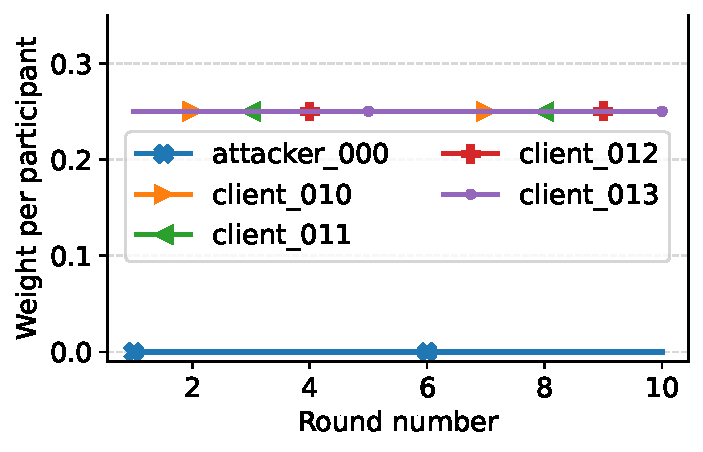
\includegraphics[width=0.65\linewidth]{./figures/eval/reput/lone_loud_expanded.pdf}
                \caption{Participants reputation for\\
                \texttt{Lone 100T}}
      \end{figure}
    \end{minipage}  
  
    \end{column}
  \end{columns}
\end{frame}


%%%%%%%%%%%%    
% Targeted min   
%%%%%%%%%%%%
\begin{frame}{Handling targeted attacks}
  \begin{columns}
    \begin{column}{.4\textwidth}
      \begin{figure}
        \captionsetup{justification=centering}
        % Info à ajouter : RI 1
        % Clustering ok.
        % Animation pour le premier ajout du cercle
        \includegraphics<1>[width=\linewidth,left]{./figures/eval/clustering/clustering_min_targeted.pdf}%
        \caption{Clustering results for\\
        \texttt{colluding minority 100T}\\ 
        Rand index=0.97}
      \end{figure}
    \end{column}
  \begin{column}{.6\textwidth}
  \begin{minipage}[t][0.35\textheight]{\textwidth}
                \centering
                \begin{table}
                    \centering
                    \footnotesize
                    \setlength\tabcolsep{1ex}
                        \begin{tabularx}{.7\textwidth}{lX|ccc}
                            \toprule % ---------------------------------
                            \multicolumn{2}{c|}{{\textbf{Scenario}}}
                            & \multicolumn{1}{c}{\texttt{RADAR}} & \multicolumn{1}{c}{\texttt{FG}} & \multicolumn{1}{c|}{\texttt{FC}} \\
                            \midrule % ---------------------------------
                            \multicolumn{2}{l|}{\textbf{Benign}}& \hg 0.00 & \ho 5.17 & \hg 0.09  \\
                            % % TARGETED ATTACKS
                            \multicolumn{2}{l|}{\textbf{Targeted} (\texttt{100T})}  & & & \\    
                            & \texttt{Lone} &\hg 0.00  & \hr 93.82 & \ho 0.45 \\
                            & \texttt{Collud. min.} & \hg 0.00 & \hg 2.97 & \hr 53.40 \\
                        \end{tabularx}
                \end{table}
        \end{minipage}
        % \vspace{0.25cm}            
    \begin{minipage}[t][0.65\textheight]{\textwidth}
        \begin{figure}
        % Matérialiser le zoom du cluster rouge vers les courbes de droites ?  
            \captionsetup{justification=centering}
                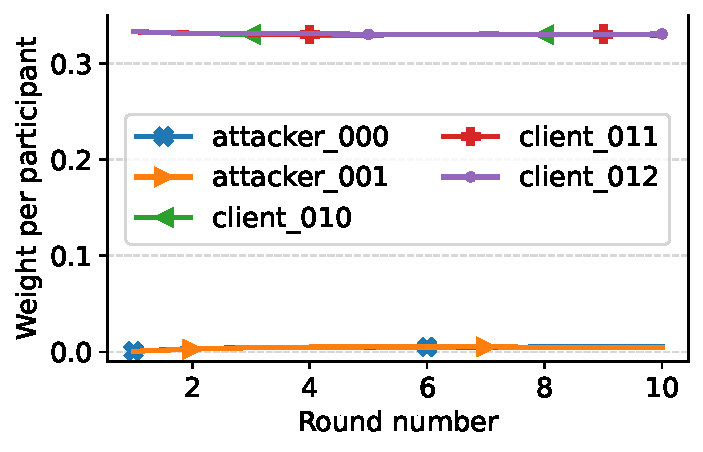
\includegraphics[width=0.65\linewidth]{./figures/eval/reput/byzantine_minority_loud_expanded.pdf}
                \caption{Participants reputation for\\
                \texttt{colluding minority 100T}}
      \end{figure}
    \end{minipage}  

  
         \end{column}
  \end{columns}
\end{frame}
%%%%%%%%%%%%    
% Targeted maj   
%%%%%%%%%%%%
\begin{frame}{Handling targeted attacks}
  \begin{columns}
    \begin{column}{.4\textwidth}
      \begin{figure}
        \captionsetup{justification=centering}
        % Info à ajouter : RI 1
        % Clustering ok.
        % Animation pour le premier ajout du cercle + le R1 = 1 ? 
        \includegraphics<1>[width=\linewidth,left]{./figures/eval/clustering/clustering_maj_targeted.pdf}%
        \caption{Clustering results for \texttt{colluding majority 100T}\\ 
        Rand index=0.96}
      \end{figure}
    \end{column}
  \begin{column}{.6\textwidth}

  \begin{minipage}[t][0.35\textheight]{\textwidth}
                \centering
                \begin{table}
                    \centering
                    \footnotesize
                    \setlength\tabcolsep{1ex}
                        \begin{tabularx}{.7\textwidth}{lX|ccc}
                            \toprule % ---------------------------------
                            \multicolumn{2}{c|}{{\textbf{Scenario}}}
                            & \multicolumn{1}{c}{\texttt{RADAR}} & \multicolumn{1}{c}{\texttt{FG}} & \multicolumn{1}{c|}{\texttt{FC}} \\
                            \midrule % ---------------------------------
                            \multicolumn{2}{l|}{\textbf{Benign}}& \hg 0.00 & \ho 5.17 & \hg 0.09  \\
                            % % TARGETED ATTACKS
                            \multicolumn{2}{l|}{\textbf{Targeted} (\texttt{100T})}  & & & \\    
                            & \texttt{Lone} &\hg 0.00  & \hr 93.82 & \ho 0.45 \\
                            & \texttt{Collud. min.} & \hg 0.00 & \hg 2.97 & \hr 53.40 \\
                            & \texttt{Collud. maj.} &  \hr 73.39 & \ho 8.10 & \hr 59.36 \\
                        \end{tabularx}
                \end{table}
        \end{minipage}
        % \vspace{0.25cm}            
    \begin{minipage}[t][0.65\textheight]{\textwidth}
        \begin{figure}
        % Matérialiser le zoom du cluster rouge vers les courbes de droites ?  
            \captionsetup{justification=centering}
                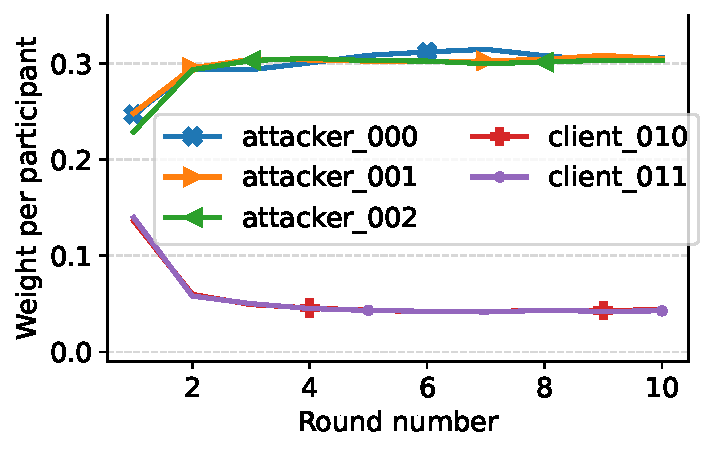
\includegraphics[width=0.65\linewidth]{./figures/eval/reput/byzantine_majority_loud_expanded.pdf}
                \caption{Participants reputation for\\
                \texttt{colluding majority 100T}}
      \end{figure}
    \end{minipage}  
         \end{column}
  \end{columns}
\end{frame}


%% Dummy frame 
% \section{Results}
% \begin{frame}{Handling heterogeneity}
%   \begin{columns}
%     \begin{column}{.4\textwidth}
%       \begin{figure}
%         % Info à ajouter : RI 1
%         % Clustering ok.
%         % Animation pour le premier ajout du cercle + le R1 = 1 ? 
%         \includegraphics<1>[width=\linewidth,left]{./figures/eval/clustering_untargeted_min.pdf}%
%         \caption{Clustering results without poisoning.}
%       \end{figure}
%     \end{column}
%   \begin{column}{.6\textwidth}

% \begin{table}
%     \centering
%     % \caption{
%     % }
%     \footnotesize
%     \setlength\tabcolsep{1ex}
%     \begin{tabularx}{.7\textwidth}{lX|ccc}
%       \toprule % ---------------------------------
%       \multicolumn{2}{c|}{{\textbf{Scenario}}}
%       & \multicolumn{1}{c}{\texttt{RADAR}} & \multicolumn{1}{c}{\texttt{FG}} & \multicolumn{1}{c|}{\texttt{FC}} \\
%       \midrule % ---------------------------------
%       \multicolumn{2}{l|}{\textbf{Benign}}& \textbf{0.00} & 5.17 &  0.09  \\

%       % TARGETED ATTACKS
%       % \multicolumn{2}{l|}{\textbf{Targeted} (\texttt{100U})}  & & & \\                  
%                   % & \texttt{Lone} &  \textbf{0.00} & 93.82 & 6.73 &  0.45 \\
%                   % & \texttt{Collud. min.} &  \textbf{0.00} &  2.97 & 9.99 & 53.40 \\
%                   % & \texttt{Collud. maj.} &  73.39 & \textbf{8.10} & 17.65 & 59.36 \\
%       % \midrule % ---------------------------------
%       % % UNTARGETED ATTACKS
%       % \multicolumn{2}{l|}{\textbf{Untargeted} (\texttt{100U})}  & & & \\
%       % & \texttt{Benign} &  0.09  & 0.39 & 33.30 & \textbf{0.06} \\
%       % & \texttt{Lone} & \textbf{0.08} & 99.89 & 54.70 & 0.12 \\
%       % & \texttt{Collud. min.} &  0.10 & \textbf{0.04} & 44.53 & 6.26 \\
%       % & \texttt{Collud. maj.} &  \textbf{0.08} & 38.98 & 59.49 & 94.36 \\          
%       % \bottomrule % ---------------------------------
%       % \small & \multicolumn{1}{c}{} & \multicolumn{4}{c}{\emph{lower is better}}
%     \end{tabularx}
%   \end{table}
  
%          \end{column}
%   \end{columns}
% \end{frame}

